\newpage
\section{Evaluation}
\label{sec:evaluation}
\subsection{Determination of the Threshold Current}
As stated in \ref{sec:threshold}
\begin{figure}[ht]
    \centering
    \begin{subfigure}{0.49\textwidth}
        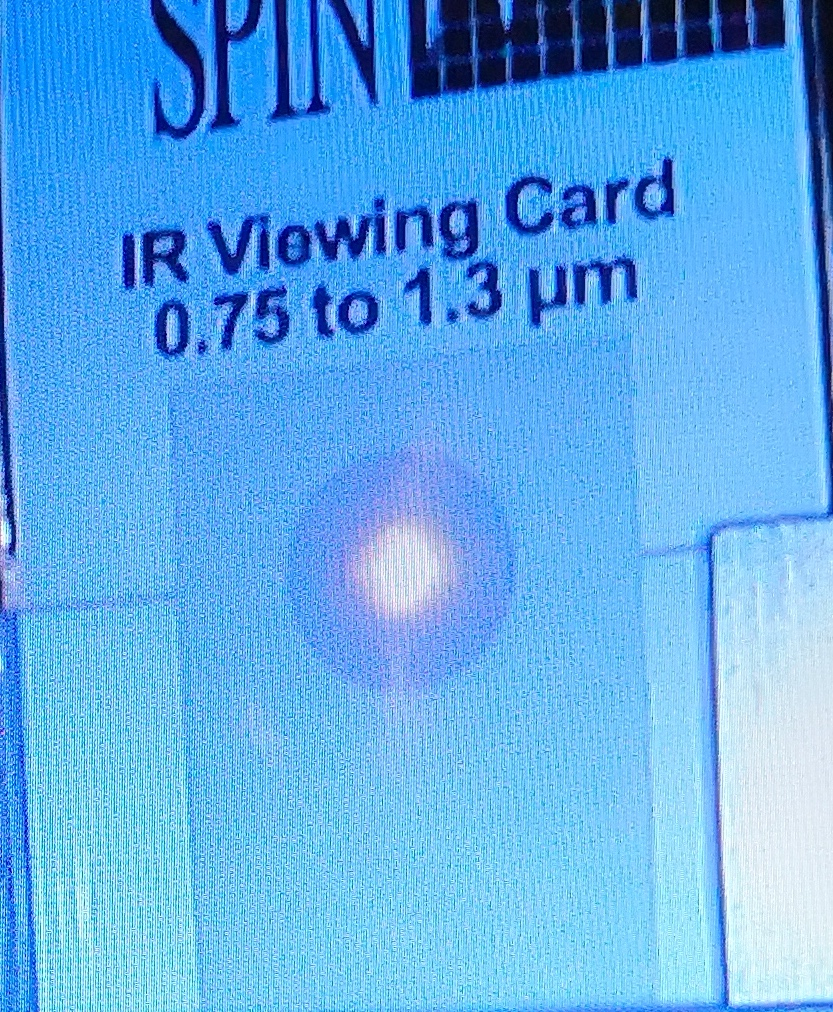
\includegraphics[width=\textwidth]{bilder/laser_before.jpg}
        \caption{The light spot on the card before lasing happens at a current below $I_\text{th}$. \cite{anleitungHeNe}}
        \label{fig:laser_before}
    \end{subfigure}
    \hfill
    \begin{subfigure}{0.49\textwidth}
        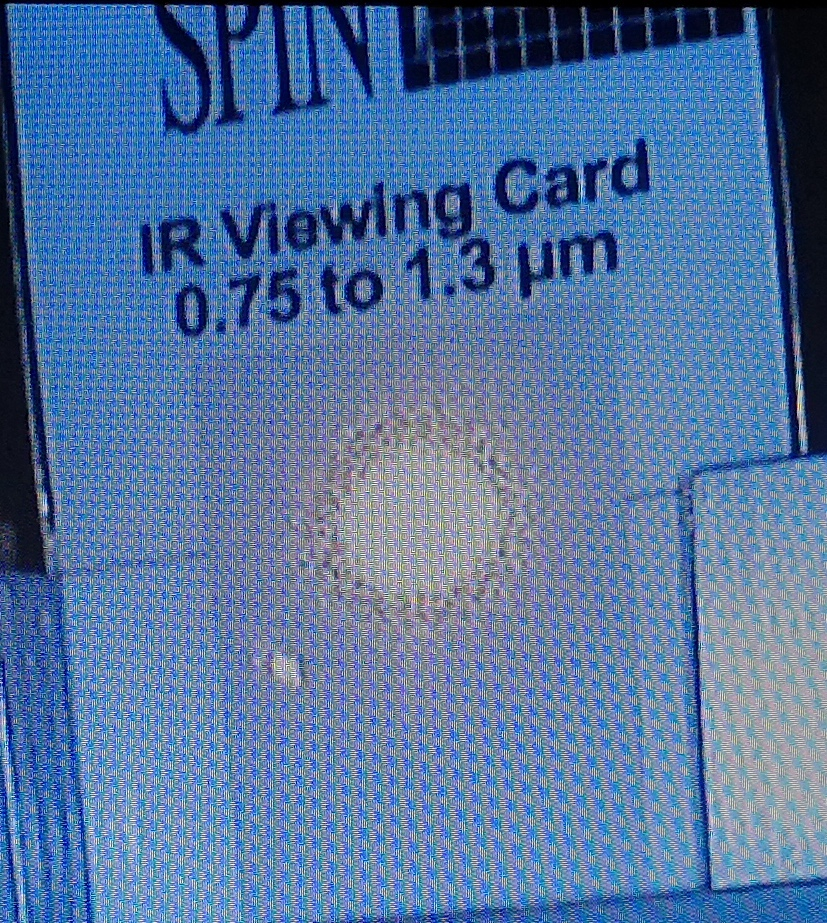
\includegraphics[width=\textwidth]{bilder/laser_after.jpg}
        \caption{The light spot on the card at the threshold current $I_\text{th}$. The laser granulation is seen on the card. \cite{anleitungHeNe}}
        \label{fig:laser_after}
    \end{subfigure}
    \caption{The light spot caused by the diode laser before and after lasing.}
\end{figure}


\subsection{Rubidium fluorescence}

\begin{figure}[ht]
    \center
    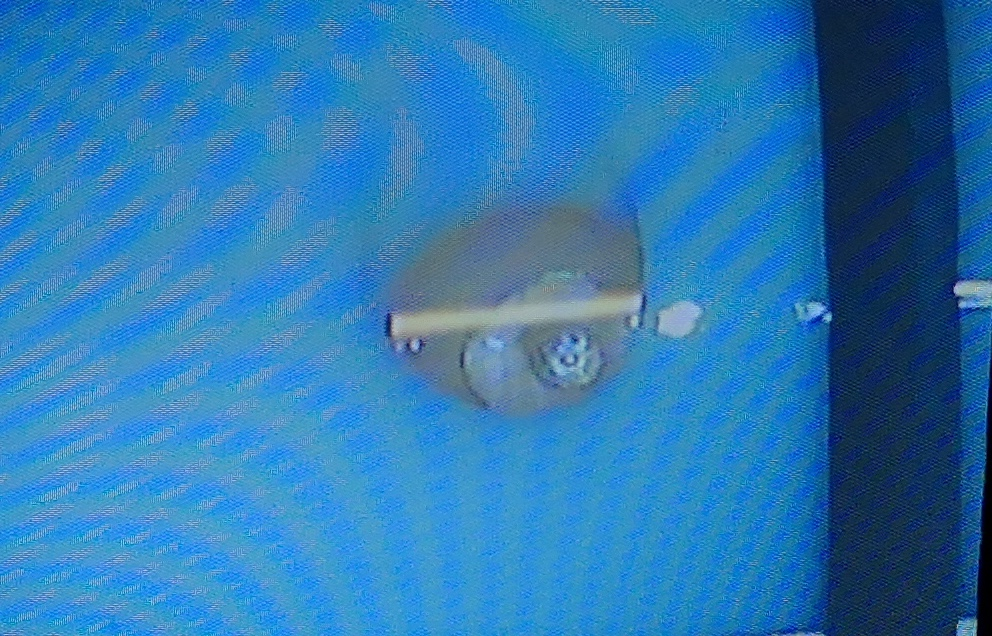
\includegraphics[width=0.8\textwidth]{bilder/fluorescence.jpg}
    \caption{The rubidium fluorescence which is seen when the diode laser reaches the necessary energy to excite the rubidium gas. \cite{anleitungHeNe}}
    \label{fig:fluorescence}
\end{figure}


\subsection{Absorption spectrum of Rubidium}

\begin{figure}[ht]
    \center
    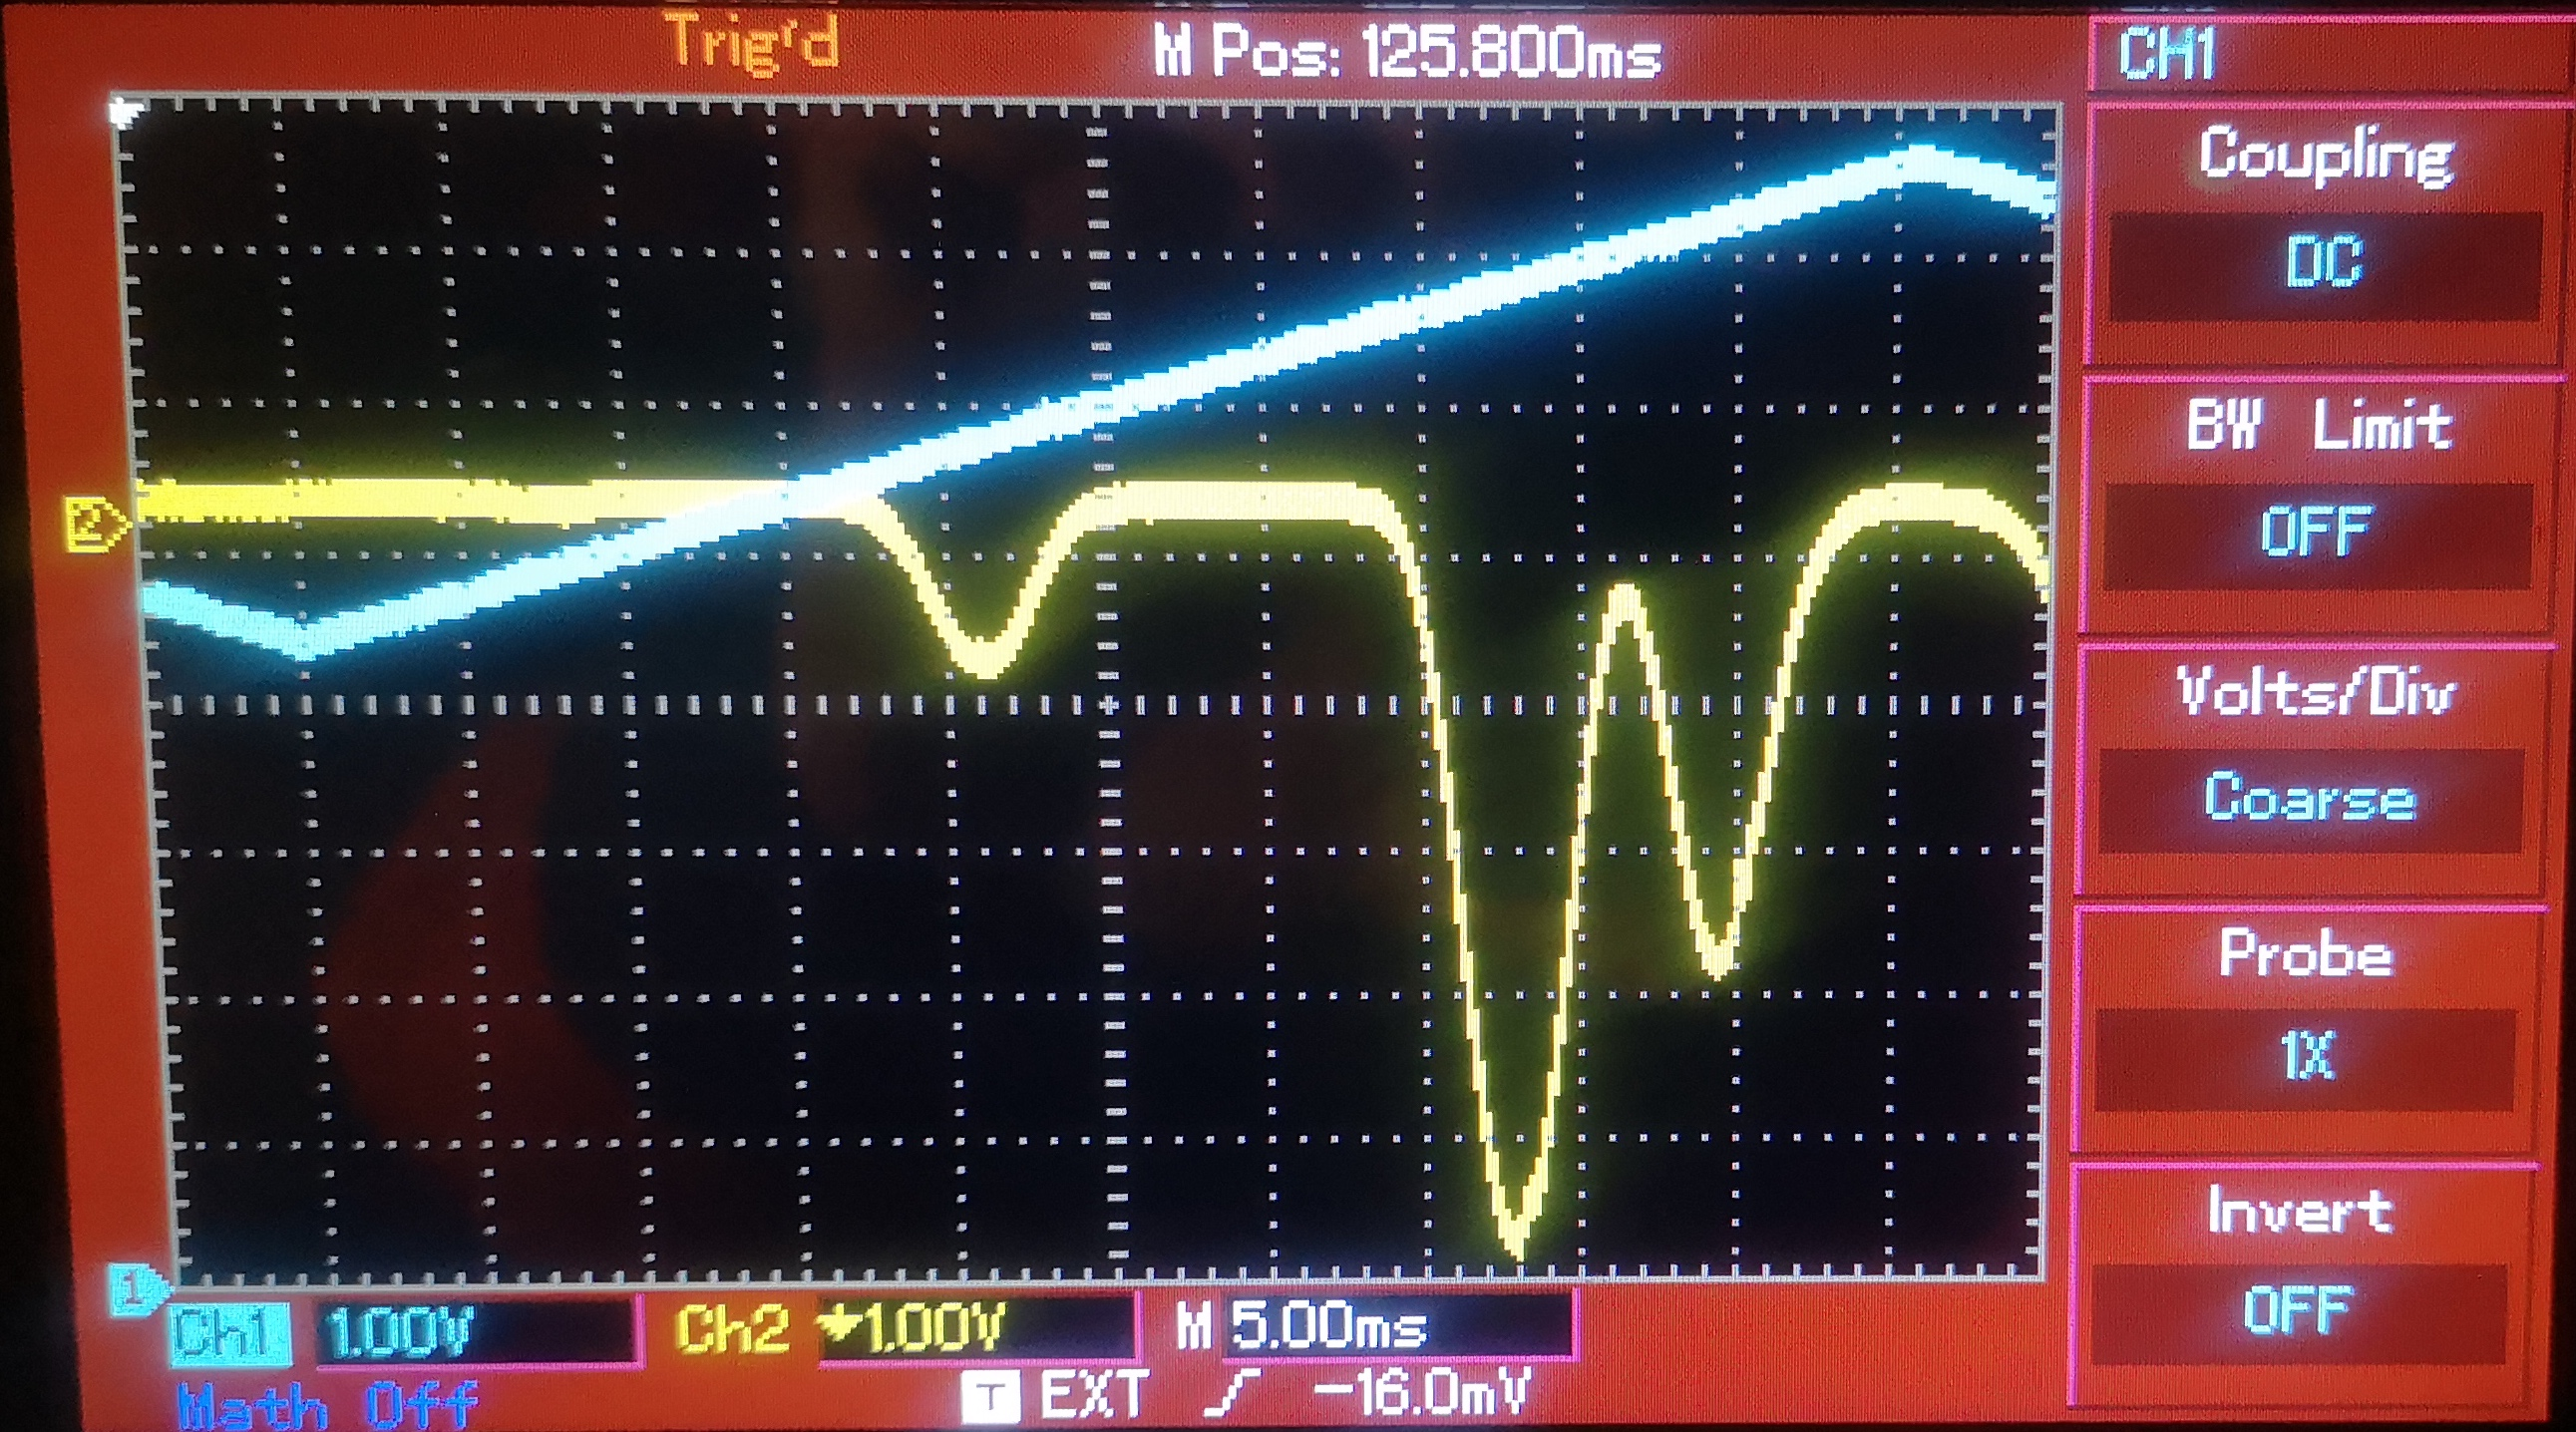
\includegraphics[width=0.8\textwidth]{bilder/spectrum.jpg}
    \caption{The absorption spectrum of rubidium containing the peaks belonging to 85a, 85b, 87a and 87b after the adjustment of the laser parameters. \cite{anleitungHeNe}}
    \label{fig:spectrum}
\end{figure}